% Created 2021-02-07 Sun 17:52
% Intended LaTeX compiler: pdflatex
\documentclass[11pt]{article}
\usepackage[utf8]{inputenc}
\usepackage[T1]{fontenc}
\usepackage{graphicx}
\usepackage{grffile}
\usepackage{longtable}
\usepackage{wrapfig}
\usepackage{rotating}
\usepackage[normalem]{ulem}
\usepackage{amsmath}
\usepackage{textcomp}
\usepackage{amssymb}
\usepackage{capt-of}
\usepackage{hyperref}
\usepackage{minted}
\usepackage[a4paper,margin=20mm]{geometry}
\usepackage{amsmath}
\usepackage{amsfonts}
\usepackage{stmaryrd}
\usepackage{bm}
\usepackage{minted}
\usemintedstyle{emacs}
\usepackage[T1]{fontenc}
\usepackage[scaled]{beraserif}
\usepackage[scaled]{berasans}
\usepackage[scaled]{beramono}
\newcommand{\tr}{\textsf{T}}
\newcommand{\grad}{\bm{\nabla}}
\newcommand{\av}[2][]{\mathbb{E}_{#1\!}\left[ #2 \right]}
\newcommand{\Prob}[2][]{\mathbb{P}_{#1\!}\left[ #2 \right]}
\newcommand{\logg}[1]{\log\!\left( #1 \right)}
\newcommand{\pred}[1]{\left\llbracket { \small #1} \right\rrbracket}
\newcommand{\e}[1]{{\rm e}^{#1}}
\newcommand{\dd}{\mathrm{d}}
\DeclareMathAlphabet{\mat}{OT1}{cmss}{bx}{n}
\newcommand{\normal}[2]{\mathcal{N}\!\left(#1 \big| #2 \right)}
\newcounter{eqCounter}
\setcounter{eqCounter}{0}
\newcommand{\explanation}{\setcounter{eqCounter}{0}\renewcommand{\labelenumi}{(\arabic{enumi})}}
\newcommand{\eq}[1][=]{\stepcounter{eqCounter}\stackrel{\text{\tiny(\arabic{eqCounter})}}{#1}}
\newcommand{\argmax}{\mathop{\mathrm{argmax}}}
\newcommand{\Dist}[2][Binom]{\mathrm{#1}\left( \strut {#2} \right)}
\author{Adam Prügel-Bennett}
\date{\today}
\title{Advanced Machine Learning Subsidary Notes\\\medskip
\large Lecture 1: When Machine Learning Works}
\hypersetup{
 pdfauthor={Adam Prügel-Bennett},
 pdftitle={Advanced Machine Learning Subsidary Notes},
 pdfkeywords={},
 pdfsubject={},
 pdfcreator={Emacs 26.3 (Org mode 9.1.9)}, 
 pdflang={English}}
\begin{document}

\maketitle


\section{Keywords}
\label{sec:orgb46b4dd}
\begin{itemize}
\item When ML Works, Bias Variance
\end{itemize}


\section{Main Points}
\label{sec:orge14fcb2}

\subsection{Generalisation}
\label{sec:orgc29fde8}
\begin{itemize}
\item We train our learning machines on a finite data set
\item But we use our learning machines on unseen data
\item If we have a too simple machine we might not be able to fit the
training data and are unlikely to do well on unseen data
\begin{center}
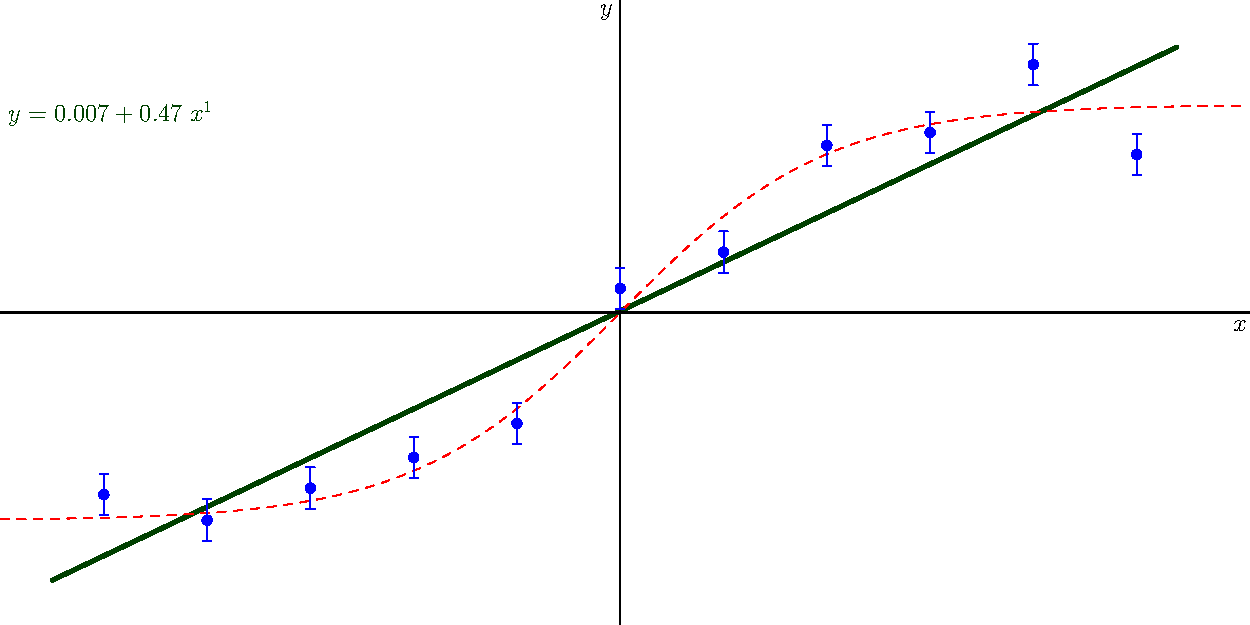
\includegraphics[width=0.4\textwidth]{figures/curveFitting-1.pdf}
\end{center}
\item If we have a too complicated machine we might be able to fit the
training data almost perfectly, but we might have learnt a too
complex rule that doesn't fit the test set
\begin{center}
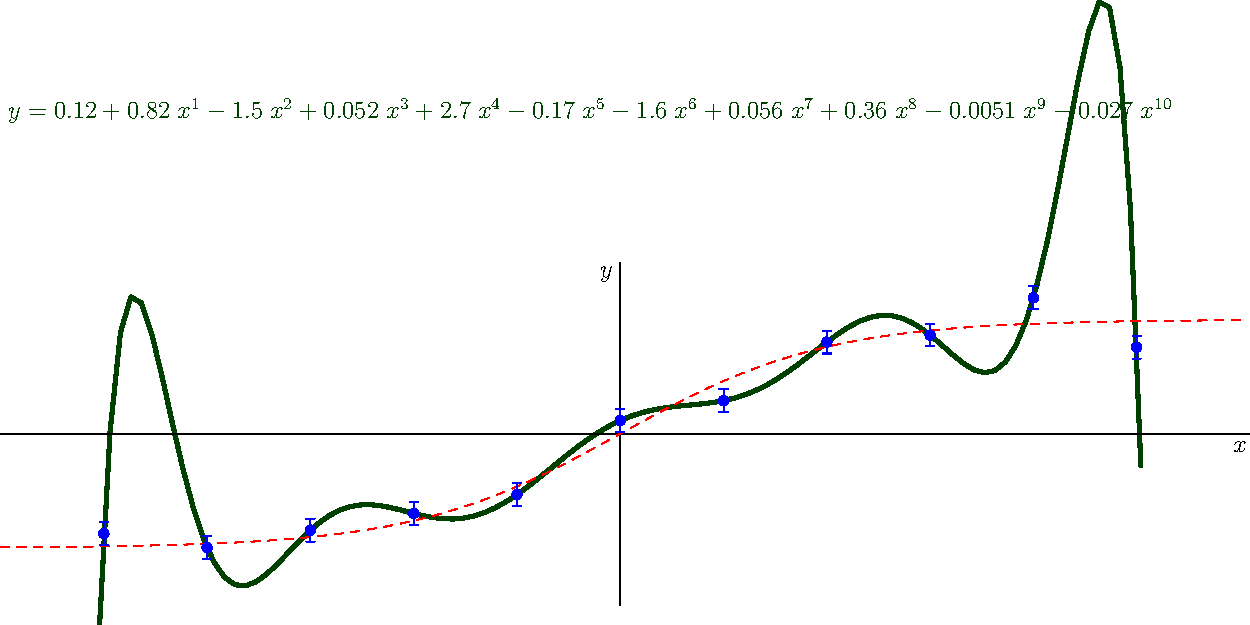
\includegraphics[width=0.4\textwidth]{figures/curveFitting-3.pdf}
\end{center}
\item Often there is a good compromise so that the learning machine
learns a simple rule that fits the training data quite well but
isn't too complicated
\begin{center}
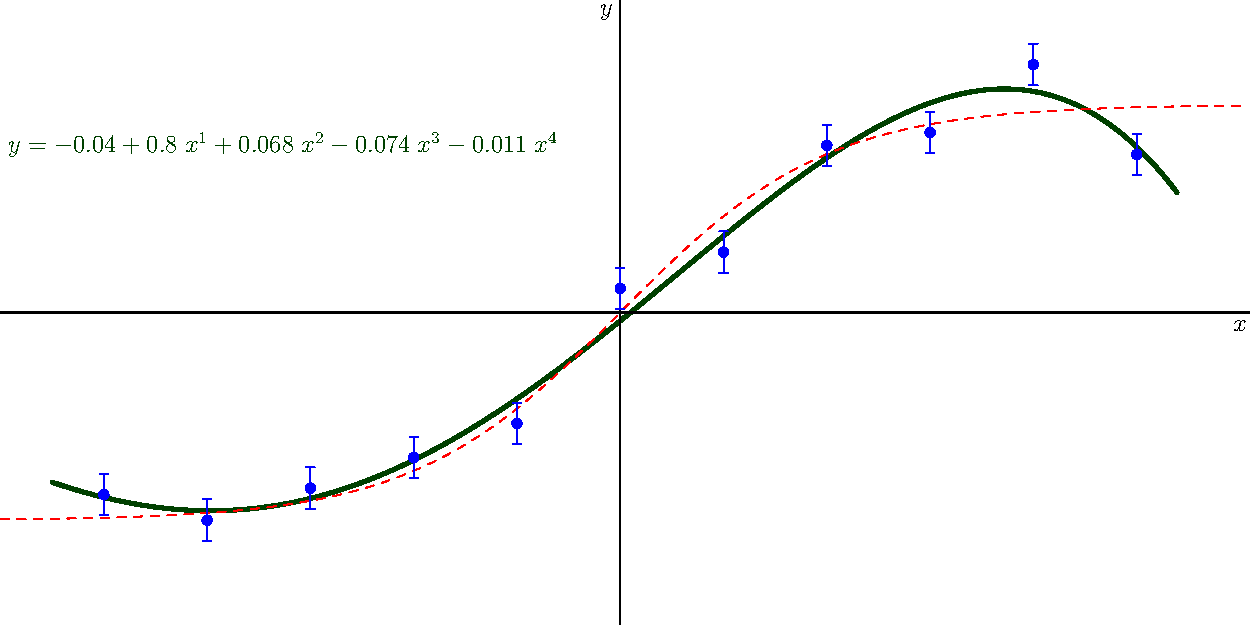
\includegraphics[width=0.4\textwidth]{figures/curveFitting-2.pdf}
\end{center}
\end{itemize}


\subsection{Bias-Variance Dilemms}
\label{sec:org31190ef}
\begin{itemize}
\item We assume that we are trying to learn some function \(f(\bm{x})\)
where \(\bm{x}\) are feature vectors
\item Our task is to learn a function \(\hat{f}\left(\bm{x} |
      \mathcal{D}\right)\) based on a training set \(\mathcal{D}\)
\item We consider a scenario where we draw different training datasets
\(\mathcal{D}\) from a distribution of training examples \(p(\bm{x})\)
\item Each training set contains \(m\) independent examples
\item We start from the definition of the \emph{mean machine}
$$  \hat{f}_m(\bm{x}) = \av[\mathcal{D}]{ \hat{f}\left(\bm{x} |
      \mathcal{D}\right)} $$
\item The mean machine makes a prediction by averaging the results of
machines trained on all possible learning datasets (clearly
this is a thought experiment and not something practical)
\item Now the \textbf{bias} is equal to generalisation performance of mean
machine
$$ B = \sum_{\bm{x}\in\mathcal{X}} p(\bm{x}) \left(
      \hat{f}_m(\bm{x}) - f(\bm{x}) \right)^2 $$
\item We consider the expected generalisation loss for a
randomly drawn dataset
\begin{itemize}
\item For any particular dataset we might do better or worse than
this expected generalisation loss
\begin{align*}
\bar{L}_G &\eq \av[\mathcal{D}]{ L_G(\mathcal{D}) } 
    \eq \av[\mathcal{D}]{  \sum_{\bm{x}\in\mathcal{X}} p(\bm{x})\,
      \left(\hat{f}(\bm{x}\vert \mathcal{D}) -
      f(\bm{x}) \right)^2}
    \\
   &\eq  \sum_{\bm{x}\in\mathcal{X}} p(\bm{x})\,
   \av[\mathcal{D}]{ 
   \left(\hat{f}(\bm{x}\vert \mathcal{D}) - f(\bm{x}) \right)^2}
   \\
  &\eq \sum_{\bm{x}\in\mathcal{X}} p(\bm{x})\, \av[\mathcal{D}]{
  \left(\left(\hat{f}(\bm{x}\vert
  \mathcal{D})
  -\hat{f}_m(\bm{x}) \right) + \left(
  \hat{f}_m(\bm{x}) - f(\bm{x})\right) \right)^2
  } \\
    &\eq  \sum_{\bm{x}\in\mathcal{X}} p(\bm{x}) \Biggl(
      \av[\mathcal{D}]{ 
      \left(\hat{f}(\bm{x}\vert \mathcal{D}) -
      \hat{f}_m(\bm{x}) \right)^2 + \left(
      \hat{f}_m(\bm{x}) - f(\bm{x}) \right)^2 }  \\
    & \hspace{5cm} + 2 \, \av[\mathcal{D}]{
      \left(\hat{f}(\bm{x}\vert \mathcal{D}) -
      \hat{f}_m(\bm{x}) \right)\left(
      \hat{f}_m(\bm{x}) - f(\bm{x}) \right) } \Biggr)
    \end{align*}
\explanation
\begin{enumerate}
\item This is the definition of the expected generalisation loss, \(\bar{L}_G\)
\item The generalisation loss is the squared difference between
the prediction of the learning machine,
\(\hat{f}(\bm{x}\vert \mathcal{D})\), and the true function,
\(f(\bm{x})\), averaged over all possible input feature vectors,
\(\bm{x}\), weighted by the probability of the input, \(p(\bm{x})\)
\item We exchange the sum and expectation
\item We add and subtract the prediction of the mean machine
\item We expand out the sum
\end{enumerate}
\item The cross term cancels
\begin{align*}
C &= \av[\mathcal{D}]{ \left(\hat{f}(\bm{x}\vert \mathcal{D}) -
   	 \hat{f}_m(\bm{x}) \right)\left(
   	 \hat{f}_m(\bm{x}) - f(\bm{x}) \right) }\\
&= \left(\av[\mathcal{D}]{\hat{f}(\bm{x}\vert \mathcal{D})} -
   	 \hat{f}_m(\bm{x}) \right)\left(
   	 \hat{f}_m(\bm{x}) - f(\bm{x}) \right)\\
&= \left(\hat{f}_m(\bm{x}) -
   	 \hat{f}_m(\bm{x}) \right)\left(
   	 \hat{f}_m(\bm{x}) - f(\bm{x}) \right) = 0
\end{align*}
\item Note we use the following properties of expectations
\begin{enumerate}
\item \(\av{A + B} = \av{A} + \av{B}\)
\item \(\av{c\,A} = c\,\av{A}\) where \(c\) doesn't depend on the
random variable you are averaging over
\item \(\av{1} = 1\)
\end{enumerate}
\item We are left with
  \begin{align*}
      \bar{L}_G &= \sum_{\bm{x}\in\mathcal{X}} p(\bm{x})
      \av[\mathcal{D}]{ 
      \left(\hat{f}(\bm{x}\vert \mathcal{D}) -
      \hat{f}_m(\bm{x}) \right)^2 + \left(
      \hat{f}_m(\bm{x}) - f(\bm{x}) \right)^2 } \\
       &= \sum_{\bm{x}\in\mathcal{X}} p(\bm{x})\, 
       \av[\mathcal{D}]{ \left(\hat{f}(\bm{x}\vert \mathcal{D}) -
      \hat{f}_m(\bm{x})\right)^2 } +
     \sum_{\bm{x}\in\mathcal{X}} p(\bm{x}) \left( \hat{f}_m(\bm{x})
- f(\bm{x}) \right)^2 
\end{align*}
\item Where we used the fact that the last term doesn't depend on
the dataset
\item The last term is equal to the bias, defined earlier as the
generalisation performance of the mean machine
\item The first term is known as the \textbf{variance}
\begin{align*}
  V = \sum_{\bm{x}\in\mathcal{X}} p(\bm{x})\,
  \av[\mathcal{D}]{ \left(\hat{f}(\bm{x}\vert \mathcal{D}) -
  \hat{f}_m(\bm{x})\right)^2 } 
\end{align*}
\item It measure how a single learning machine differs from the mean machine
\item We therefore have \(\bar{L}_G = B + V\) or
$$ \text{Expected Generalisation Loss} = \text{Bias} +
        \text{Variance} $$
\end{itemize}
\item The \textbf{Bias-Variance Dilemma} is that
\begin{itemize}
\item Simple machine are likely to have high bias
\begin{itemize}
\item because any single machine can't represent the data well the
mean machine won't be accurate
\item this is true of the curve fitting example, but it is not
true of decision trees where the average of many decision
trees can learn a far more complex division boundary than a
single machine
\end{itemize}
\item Complex machines are likely to have high variance
\begin{itemize}
\item Complex machine are likely to be sensitive to the training
data whereas simpler machines (because of their lack of
flexibility) aren't as sensitive
\end{itemize}
\end{itemize}
\item A lot of this course will be looking at machines that cleverly
resolve this dilemma
\end{itemize}

\section{Experiments}
\label{sec:org810bcb7}
Download the Jupyter Notebook

\begin{itemize}
\item This computes the training and generalisation loss as well as
the bias and variance for arbitrary functions (at least approximately)
\item We can do this because it is a 1-D function
\item See if you can understand the code
\end{itemize}

\subsection{Questions}
\label{sec:org9c42b9b}
\begin{itemize}
\item What is the effect of increasing the number of training points?
\item What is the effect of using a more complex function, E.g. \(\e{-x} \sin(x)\)?
\end{itemize}
\end{document}
